%%s Beamer template was created by Cameron Bracken.
%%  Anyone can freely use or modify it for any purpose
%%  without attribution.
%%
%%  Last Modified: January 9, 2009
%%

\documentclass[xcolor=x11names,compress]{beamer}

%% General document %%%%%%%%%%%%%%%%%%%%%%%%%%%%%%%%%%
\usepackage{graphicx}
\usepackage{tikz}
\usetikzlibrary{decorations.fractals}
%%%%%%%%%%%%%%%%%%%%%%%%%%%%%%%%%%%%%%%%%%%%%%%%%%%%%%

%% Color Definitions%%%%%%%%%%%%%%%%%%%%%%%%%%%%%%%%%%
\definecolor{pinegreen}{rgb}{0.0, 0.47, 0.44}
\definecolor{charcoal}{rgb}{0.21, 0.27, 0.31}
\definecolor{viridian}{rgb}{0.25, 0.51, 0.43}
\definecolor{rust}{rgb}{0.72, 0.25, 0.05}
\definecolor{taupegray}{rgb}{0.55, 0.52, 0.54}
\definecolor{tomato}{rgb}{1.0,  0.38823529,  0.27843137}
\definecolor{dodgerblue}{rgb}{0.11764706,  0.56470588,  1.0}
\definecolor{darkcoral}{rgb}{0.8, 0.36, 0.27}
%%%%%%%%%%%%%%%%%%%%%%%%%%%%%%%%%%%%%%%%%%%%%%%%%%%%%%


%% Beamer Layout %%%%%%%%%%%%%%%%%%%%%%%%%%%%%%%%%%
\useoutertheme[subsection=false,shadow]{miniframes}
\useinnertheme{default}
%\usefonttheme{serif}
\usepackage[sfdefault,light]{roboto}  %% Option 'sfdefault' only if the base font of the document is to be sans serif
\usepackage[T1]{fontenc}
\usepackage{palatino}
\usepackage{braket}
\setbeamertemplate{navigation symbols}{}
\setbeamertemplate{footline}[frame number]
\setbeamerfont{title like}{shape=\scshape}
\setbeamerfont{frametitle}{shape=\scshape}
\setbeamerfont{footnote}{size=\small}
\setbeamercolor*{lower separation line head}{bg=pinegreen}
\setbeamercolor*{normal text}{fg=black,bg=white}
\setbeamercolor*{alerted text}{fg=red}
\setbeamercolor*{example text}{fg=black}
\setbeamercolor*{structure}{fg=black}
\setbeamercolor*{palette tertiary}{fg=black,bg=black!5}
\setbeamercolor*{palette quaternary}{fg=black,bg=black!10}
\usepackage[listings,theorems]{tcolorbox}
%% Packages%%%%%%%%%%%%%%%%%%%%%%%%%%%%%%%%%%
\usepackage{soul}
\usepackage[style=chem-acs]{biblatex}
\bibliography{qmc_solids.bib}
\usepackage{listings}
%set up math font
\usepackage{amsmath}
\usepackage{mathpazo}
\renewcommand\rmdefault{lmr}
% all tikz packages for images
\usepackage{tikz}
\usepackage{tikzorbital}
\usetikzlibrary{arrows,shapes}
\tikzstyle{every picture}+=[remember picture]
\usepackage{graphicx}
% otherstuff
\usepackage{booktabs}
\usepackage{siunitx} % unit stuff
\usepackage{cancel} % to cross out stuff
\usepackage{modiagram}
\usepackage[version=3]{mhchem}
\usepackage{enumitem} % needed to have symbol in itemize in this template
\usepackage{array} %used for something in the template
\usepackage{hyperref} % url

%%%%%%%%%%%%%%%%%%%%%%%%%%%%%%%%%%%%%%%%%%%%%%%%%%%%%%

\renewcommand{\(}{\begin{columns}}
\renewcommand{\)}{\end{columns}}
\newcommand{\<}[1]{\begin{column}{#1}}
\renewcommand{\>}{\end{column}}

\title[{\makebox[.5\paperwidth]{General Chemistry Recitation 1\hfill
       \insertframenumber/\inserttotalframenumber}}]{ICE-T Day 1:\\
Python introduction}
\author[\quad Amanda \quad\quad\quad\quad aed63@pitt.edu]{
}

\date{\small{\today}}


\begin{document}

%%%%%%%%%%%%%%%%%%%%%%%%%%%%%%%%%%%%%%%%%%%%%%%%%%%%%%
\section{Introduction}
\begin{frame}
\titlepage
\end{frame}
%%%%%%%%%%%%%%%%%%%%%%%%%%%%%%%%%%%%%%%%%%%%%%%%%%%%%%
%%%%%%%%%%%%%%%%%%%%%%%%%%%%%%%%%%%%%%%%%%%%%%%%%%%%%%
\begin{frame}{Programming Hierarchy}
    \begin{center}
    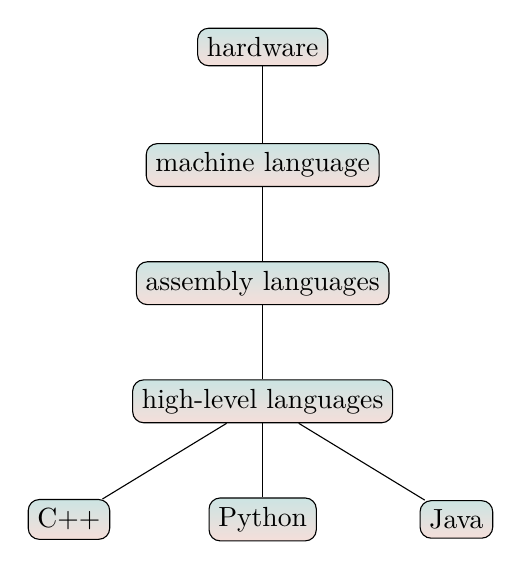
\begin{tikzpicture}[sibling distance=7em, every node/.style = {shape=rectangle, rounded corners, draw, align=center, top color=pinegreen!20, bottom color=darkcoral!20}]
      \node {hardware}
        child { node {machine language}
          child { node {assembly languages}
            child { node {high-level languages}
            child { node {C++} }
            child { node {Python} }
            child { node {Java} }
            }
            }
            };
    \end{tikzpicture}
\end{center}
\end{frame}
%%%%%%%%%%%%%%%%%%%%%%%%%%%%%%%%%%%%%%%%%%%%%%%%%%%%%%
%%%%%%%%%%%%%%%%%%%%%%%%%%%%%%%%%%%%%%%%%%%%%%%%%%%%%%
    \begin{frame}{Why Python?}

\includegraphics[width= 0.4\textwidth]{python-logo-master-flat}
\begin{enumerate}[label=$\bullet$]
\item<1-> \textcolor{darkcoral}{beginner friendly: } \textcolor<2->{gray!30}{tutorials, community, quick!}
\item<2-> \textcolor{darkcoral}{easy to understand:} \textcolor<3->{gray!30}{reads like english}
\item<3-> \textcolor{darkcoral}{flexibility:} \textcolor<4->{gray!30}{dynamic, forgiving}
\item<4-> \textcolor{darkcoral}{career opportunities:} \textcolor<5->{gray}{2nd most demanded skill with highest average salary.\cite{http://www.bestprogramminglanguagefor.me/why-learn-python}}
\end{enumerate}
\end{frame}

%%%%%%%%%%%%%%%%%%%%%%%%%%%%%%%%%%%%%%%%%%%%%%%%%%%%%%
%%%%%%%%%%%%%%%%%%%%%%%%%%%%%%%%%%%%%%%%%%%%%%%%%%%%%%
\begin{frame}{Where to begin?}
    \begin{center}
    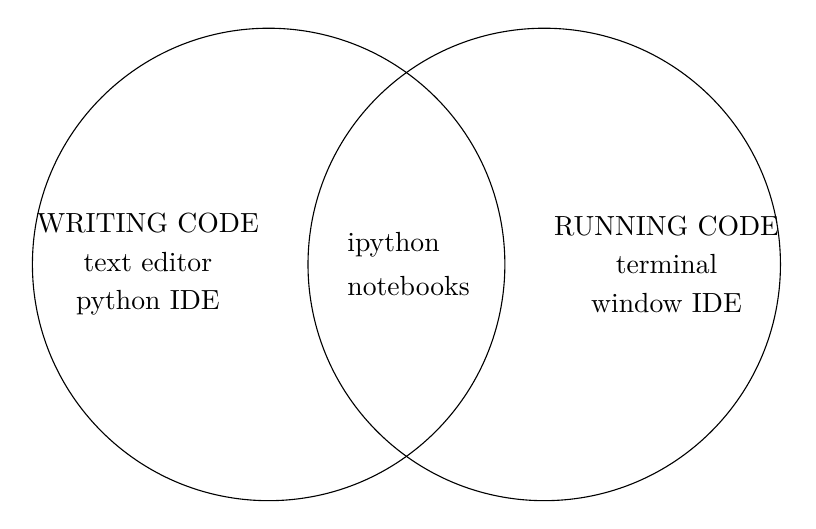
\begin{tikzpicture}
        % \fill[gray] (0,0) circle (3cm);
        % \fill[blue] (1.5,0) circle (3cm);
        \draw (0,0) circle (3cm) node [left, rectangle split, rectangle split parts = 3] {WRITING CODE \nodepart{second} text editor\nodepart{third} python IDE}
        ;
        \node[text width=2cm, rectangle split, rectangle split parts = 2] at (2,0) {ipython \nodepart{second} notebooks};
        \draw (3.5,0) circle (3cm) node [right, rectangle split, rectangle split parts = 3]{RUNNING CODE \nodepart{second} terminal \nodepart{third} window IDE};
    \end{tikzpicture}
\end{center}
\end{frame}
%%%%%%%%%%%%%%%%%%%%%%%%%%%%%%%%%%%%%%%%%%%%%%%%%%%%%%
%%%%%%%%%%%%%%%%%%%%%%%%%%%%%%%%%%%%%%%%%%%%%%%%%%%%%%
\begin{frame}
    \begin{center}
        \large{www.github.com}
        \begin{align*}
        \text{username} = & \text{firstname\_lastname}\\
         &  \text{example: amanda\_dumi}\\
        \end{align*}

        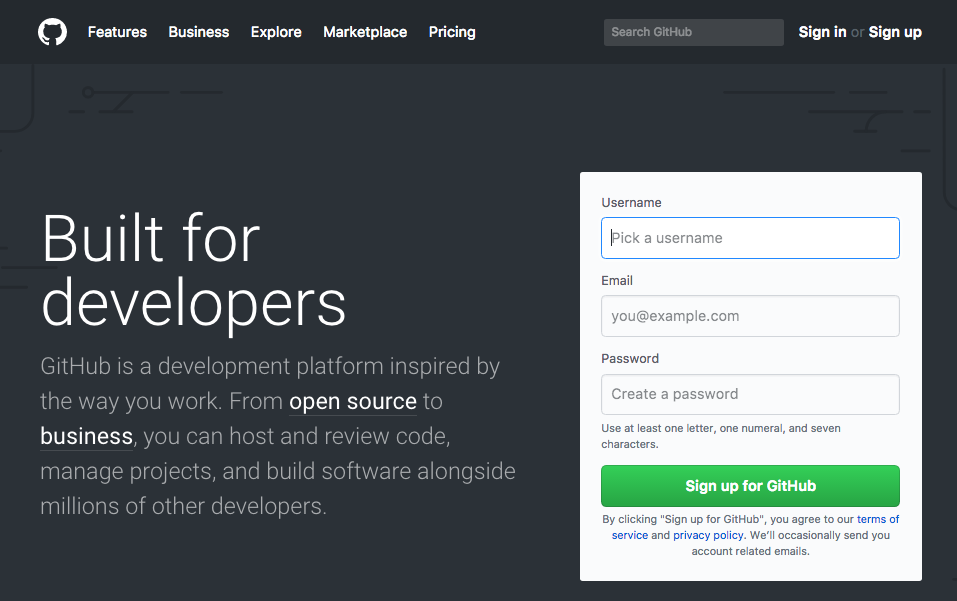
\includegraphics[width= 0.8\textwidth]{github_webpage}
    \end{center}
\end{frame}
\end{document}
